% Options for packages loaded elsewhere
\PassOptionsToPackage{unicode}{hyperref}
\PassOptionsToPackage{hyphens}{url}
%
\documentclass[
]{article}
\usepackage{amsmath,amssymb}
\usepackage{lmodern}
\usepackage{iftex}
\ifPDFTeX
  \usepackage[T1]{fontenc}
  \usepackage[utf8]{inputenc}
  \usepackage{textcomp} % provide euro and other symbols
\else % if luatex or xetex
  \usepackage{unicode-math}
  \defaultfontfeatures{Scale=MatchLowercase}
  \defaultfontfeatures[\rmfamily]{Ligatures=TeX,Scale=1}
\fi
% Use upquote if available, for straight quotes in verbatim environments
\IfFileExists{upquote.sty}{\usepackage{upquote}}{}
\IfFileExists{microtype.sty}{% use microtype if available
  \usepackage[]{microtype}
  \UseMicrotypeSet[protrusion]{basicmath} % disable protrusion for tt fonts
}{}
\makeatletter
\@ifundefined{KOMAClassName}{% if non-KOMA class
  \IfFileExists{parskip.sty}{%
    \usepackage{parskip}
  }{% else
    \setlength{\parindent}{0pt}
    \setlength{\parskip}{6pt plus 2pt minus 1pt}}
}{% if KOMA class
  \KOMAoptions{parskip=half}}
\makeatother
\usepackage{xcolor}
\usepackage[margin=1in]{geometry}
\usepackage{color}
\usepackage{fancyvrb}
\newcommand{\VerbBar}{|}
\newcommand{\VERB}{\Verb[commandchars=\\\{\}]}
\DefineVerbatimEnvironment{Highlighting}{Verbatim}{commandchars=\\\{\}}
% Add ',fontsize=\small' for more characters per line
\usepackage{framed}
\definecolor{shadecolor}{RGB}{248,248,248}
\newenvironment{Shaded}{\begin{snugshade}}{\end{snugshade}}
\newcommand{\AlertTok}[1]{\textcolor[rgb]{0.94,0.16,0.16}{#1}}
\newcommand{\AnnotationTok}[1]{\textcolor[rgb]{0.56,0.35,0.01}{\textbf{\textit{#1}}}}
\newcommand{\AttributeTok}[1]{\textcolor[rgb]{0.77,0.63,0.00}{#1}}
\newcommand{\BaseNTok}[1]{\textcolor[rgb]{0.00,0.00,0.81}{#1}}
\newcommand{\BuiltInTok}[1]{#1}
\newcommand{\CharTok}[1]{\textcolor[rgb]{0.31,0.60,0.02}{#1}}
\newcommand{\CommentTok}[1]{\textcolor[rgb]{0.56,0.35,0.01}{\textit{#1}}}
\newcommand{\CommentVarTok}[1]{\textcolor[rgb]{0.56,0.35,0.01}{\textbf{\textit{#1}}}}
\newcommand{\ConstantTok}[1]{\textcolor[rgb]{0.00,0.00,0.00}{#1}}
\newcommand{\ControlFlowTok}[1]{\textcolor[rgb]{0.13,0.29,0.53}{\textbf{#1}}}
\newcommand{\DataTypeTok}[1]{\textcolor[rgb]{0.13,0.29,0.53}{#1}}
\newcommand{\DecValTok}[1]{\textcolor[rgb]{0.00,0.00,0.81}{#1}}
\newcommand{\DocumentationTok}[1]{\textcolor[rgb]{0.56,0.35,0.01}{\textbf{\textit{#1}}}}
\newcommand{\ErrorTok}[1]{\textcolor[rgb]{0.64,0.00,0.00}{\textbf{#1}}}
\newcommand{\ExtensionTok}[1]{#1}
\newcommand{\FloatTok}[1]{\textcolor[rgb]{0.00,0.00,0.81}{#1}}
\newcommand{\FunctionTok}[1]{\textcolor[rgb]{0.00,0.00,0.00}{#1}}
\newcommand{\ImportTok}[1]{#1}
\newcommand{\InformationTok}[1]{\textcolor[rgb]{0.56,0.35,0.01}{\textbf{\textit{#1}}}}
\newcommand{\KeywordTok}[1]{\textcolor[rgb]{0.13,0.29,0.53}{\textbf{#1}}}
\newcommand{\NormalTok}[1]{#1}
\newcommand{\OperatorTok}[1]{\textcolor[rgb]{0.81,0.36,0.00}{\textbf{#1}}}
\newcommand{\OtherTok}[1]{\textcolor[rgb]{0.56,0.35,0.01}{#1}}
\newcommand{\PreprocessorTok}[1]{\textcolor[rgb]{0.56,0.35,0.01}{\textit{#1}}}
\newcommand{\RegionMarkerTok}[1]{#1}
\newcommand{\SpecialCharTok}[1]{\textcolor[rgb]{0.00,0.00,0.00}{#1}}
\newcommand{\SpecialStringTok}[1]{\textcolor[rgb]{0.31,0.60,0.02}{#1}}
\newcommand{\StringTok}[1]{\textcolor[rgb]{0.31,0.60,0.02}{#1}}
\newcommand{\VariableTok}[1]{\textcolor[rgb]{0.00,0.00,0.00}{#1}}
\newcommand{\VerbatimStringTok}[1]{\textcolor[rgb]{0.31,0.60,0.02}{#1}}
\newcommand{\WarningTok}[1]{\textcolor[rgb]{0.56,0.35,0.01}{\textbf{\textit{#1}}}}
\usepackage{graphicx}
\makeatletter
\def\maxwidth{\ifdim\Gin@nat@width>\linewidth\linewidth\else\Gin@nat@width\fi}
\def\maxheight{\ifdim\Gin@nat@height>\textheight\textheight\else\Gin@nat@height\fi}
\makeatother
% Scale images if necessary, so that they will not overflow the page
% margins by default, and it is still possible to overwrite the defaults
% using explicit options in \includegraphics[width, height, ...]{}
\setkeys{Gin}{width=\maxwidth,height=\maxheight,keepaspectratio}
% Set default figure placement to htbp
\makeatletter
\def\fps@figure{htbp}
\makeatother
\setlength{\emergencystretch}{3em} % prevent overfull lines
\providecommand{\tightlist}{%
  \setlength{\itemsep}{0pt}\setlength{\parskip}{0pt}}
\setcounter{secnumdepth}{-\maxdimen} % remove section numbering
\usepackage{booktabs}
\usepackage{longtable}
\usepackage{array}
\usepackage{multirow}
\usepackage{wrapfig}
\usepackage{float}
\usepackage{colortbl}
\usepackage{pdflscape}
\usepackage{tabu}
\usepackage{threeparttable}
\usepackage{threeparttablex}
\usepackage[normalem]{ulem}
\usepackage{makecell}
\usepackage{xcolor}
\usepackage{siunitx}
\newcolumntype{d}{S[input-symbols = ()]}
\ifLuaTeX
  \usepackage{selnolig}  % disable illegal ligatures
\fi
\IfFileExists{bookmark.sty}{\usepackage{bookmark}}{\usepackage{hyperref}}
\IfFileExists{xurl.sty}{\usepackage{xurl}}{} % add URL line breaks if available
\urlstyle{same} % disable monospaced font for URLs
\hypersetup{
  pdftitle={Assignment 1},
  hidelinks,
  pdfcreator={LaTeX via pandoc}}

\title{Assignment 1}
\author{}
\date{\vspace{-2.5em}2022-10-05}

\begin{document}
\maketitle

\begin{Shaded}
\begin{Highlighting}[]
\NormalTok{name }\OtherTok{\textless{}{-}} \FunctionTok{Sys.info}\NormalTok{()}
\NormalTok{name[}\DecValTok{7}\NormalTok{]}
\end{Highlighting}
\end{Shaded}

\begin{verbatim}
##          user 
## "husaynjessa"
\end{verbatim}

\begin{Shaded}
\begin{Highlighting}[]
\DocumentationTok{\#\#\# Load the packages we will need for this file \#\#\#\#}

\FunctionTok{library}\NormalTok{(tidyverse) }\CommentTok{\# load the installed package for each new session of R}
\end{Highlighting}
\end{Shaded}

\begin{verbatim}
## -- Attaching packages --------------------------------------- tidyverse 1.3.2 --
## v ggplot2 3.3.5     v purrr   0.3.4
## v tibble  3.1.6     v dplyr   1.0.9
## v tidyr   1.1.4     v stringr 1.4.0
## v readr   2.1.2     v forcats 0.5.1
## -- Conflicts ------------------------------------------ tidyverse_conflicts() --
## x dplyr::filter() masks stats::filter()
## x dplyr::lag()    masks stats::lag()
\end{verbatim}

\begin{Shaded}
\begin{Highlighting}[]
\FunctionTok{library}\NormalTok{(broom) }\CommentTok{\# helps for storing regression output}
\FunctionTok{library}\NormalTok{(here) }\CommentTok{\# for file organization}
\end{Highlighting}
\end{Shaded}

\begin{verbatim}
## here() starts at /Users/husaynjessa/Documents/GitHub/HAD5744
\end{verbatim}

\begin{Shaded}
\begin{Highlighting}[]
\FunctionTok{library}\NormalTok{(modelsummary) }\CommentTok{\# For making regression tables}
\FunctionTok{library}\NormalTok{(psych) }\CommentTok{\# For creating summary statistics table}
\end{Highlighting}
\end{Shaded}

\begin{verbatim}
## 
## Attaching package: 'psych'
## 
## The following object is masked from 'package:modelsummary':
## 
##     SD
## 
## The following objects are masked from 'package:ggplot2':
## 
##     %+%, alpha
\end{verbatim}

\begin{Shaded}
\begin{Highlighting}[]
\FunctionTok{library}\NormalTok{(countrycode) }\CommentTok{\# Used to get continents from countries}
\FunctionTok{library}\NormalTok{(fastDummies) }\CommentTok{\# To create dummy variables}
\FunctionTok{library}\NormalTok{(vtable) }\CommentTok{\#Shows information about the variables in your data set}
\end{Highlighting}
\end{Shaded}

\begin{verbatim}
## Loading required package: kableExtra
## 
## Attaching package: 'kableExtra'
## 
## The following object is masked from 'package:dplyr':
## 
##     group_rows
\end{verbatim}

\begin{Shaded}
\begin{Highlighting}[]
\FunctionTok{library}\NormalTok{(lmtest) }\CommentTok{\#A collection of tests, data sets, and examples for diagnostic checking in linear regression models}
\end{Highlighting}
\end{Shaded}

\begin{verbatim}
## Loading required package: zoo
## 
## Attaching package: 'zoo'
## 
## The following objects are masked from 'package:base':
## 
##     as.Date, as.Date.numeric
\end{verbatim}

\begin{Shaded}
\begin{Highlighting}[]
\FunctionTok{library}\NormalTok{(flextable) }\CommentTok{\#Create pretty tables for \textquotesingle{}HTML\textquotesingle{}, \textquotesingle{}PDF\textquotesingle{}, \textquotesingle{}Microsoft Word\textquotesingle{}, \textquotesingle{}Microsoft PowerPoint\textquotesingle{} documents from \textquotesingle{}R Markdown\textquotesingle{} }
\end{Highlighting}
\end{Shaded}

\begin{verbatim}
## 
## Attaching package: 'flextable'
## 
## The following objects are masked from 'package:kableExtra':
## 
##     as_image, footnote
## 
## The following object is masked from 'package:purrr':
## 
##     compose
\end{verbatim}

\begin{Shaded}
\begin{Highlighting}[]
\CommentTok{\# set working directory}
\FunctionTok{here}\NormalTok{()}
\end{Highlighting}
\end{Shaded}

\begin{verbatim}
## [1] "/Users/husaynjessa/Documents/GitHub/HAD5744"
\end{verbatim}

\begin{Shaded}
\begin{Highlighting}[]
\NormalTok{assign\_data }\OtherTok{\textless{}{-}} \FunctionTok{read.csv}\NormalTok{(}\StringTok{"Dataset 1.csv"}\NormalTok{) }\CommentTok{\# assign data to an object}
\end{Highlighting}
\end{Shaded}

\begin{center}\rule{0.5\linewidth}{0.5pt}\end{center}

\begin{Shaded}
\begin{Highlighting}[]
\CommentTok{\# Scan through dataframe to see variable class types}
\ControlFlowTok{for}\NormalTok{(values }\ControlFlowTok{in} \FunctionTok{names}\NormalTok{(assign\_data))\{}
  \FunctionTok{print}\NormalTok{(}\FunctionTok{names}\NormalTok{(assign\_data[values]))}
\NormalTok{  name }\OtherTok{\textless{}{-}} \FunctionTok{names}\NormalTok{(assign\_data[values])}
  \FunctionTok{print}\NormalTok{(}\FunctionTok{class}\NormalTok{(assign\_data[,values]))}
\NormalTok{\}}
\end{Highlighting}
\end{Shaded}

\begin{verbatim}
## [1] "Country"
## [1] "character"
## [1] "LEBF20052"
## [1] "numeric"
## [1] "LEBM20052"
## [1] "numeric"
## [1] "maxINFM20052"
## [1] "numeric"
## [1] "GDPPCUS2005"
## [1] "numeric"
## [1] "HXPC2005"
## [1] "character"
## [1] "PctHXPUB2005"
## [1] "character"
## [1] "TotFertRate2005"
## [1] "numeric"
## [1] "AdolFertRt2005"
## [1] "character"
## [1] "FtoMPrimaryEnrl2005ONY"
## [1] "character"
## [1] "PctUrb2005"
## [1] "numeric"
## [1] "Sanitation2005ONY"
## [1] "character"
## [1] "ImprWaterUrb2005ONY"
## [1] "character"
## [1] "ImpWatRur2005ONY"
## [1] "character"
## [1] "FLFPR2005"
## [1] "character"
## [1] "MLFP2005"
## [1] "character"
## [1] "PopGr2005"
## [1] "numeric"
## [1] "PctPop0142005"
## [1] "character"
## [1] "PctPop65Pl2005"
## [1] "character"
\end{verbatim}

\begin{Shaded}
\begin{Highlighting}[]
\CommentTok{\# Convert all to character}
\NormalTok{assign\_data[, }\DecValTok{1}\SpecialCharTok{:}\DecValTok{19}\NormalTok{] }\OtherTok{\textless{}{-}} \FunctionTok{lapply}\NormalTok{(assign\_data[, }\DecValTok{1}\SpecialCharTok{:}\DecValTok{19}\NormalTok{], as.character)}

\CommentTok{\# Assign the NAs in dataset to NA}
\NormalTok{assign\_data }\OtherTok{\textless{}{-}} \FunctionTok{mutate\_at}\NormalTok{(}\AttributeTok{.tbl =}\NormalTok{ assign\_data, }
                                \AttributeTok{.vars =} \FunctionTok{vars}\NormalTok{(Country}\SpecialCharTok{:}\NormalTok{PctPop65Pl2005), }
                                \AttributeTok{.funs =} \SpecialCharTok{\textasciitilde{}}\FunctionTok{case\_when}\NormalTok{(. }\SpecialCharTok{==} \StringTok{"\#N/A"} \SpecialCharTok{\textasciitilde{}} \ConstantTok{NA\_character\_}\NormalTok{,}
\NormalTok{                                                   . }\SpecialCharTok{==} \StringTok{"{-}"} \SpecialCharTok{\textasciitilde{}} \ConstantTok{NA\_character\_}\NormalTok{,}
                                                   \ConstantTok{TRUE} \SpecialCharTok{\textasciitilde{}}\NormalTok{ .,}
                                                   \ConstantTok{TRUE} \SpecialCharTok{\textasciitilde{}} \FunctionTok{as.character}\NormalTok{(}\ConstantTok{NA\_character\_}\NormalTok{)))}

\CommentTok{\# Save cleaned data}
\FunctionTok{write.csv}\NormalTok{(assign\_data, }\StringTok{"Dataset 1\_Clean.csv"}\NormalTok{, }\AttributeTok{row.names =} \ConstantTok{FALSE}\NormalTok{)}

\CommentTok{\# Read in cleaned data}
\NormalTok{Dataset1 }\OtherTok{\textless{}{-}} \FunctionTok{read.csv}\NormalTok{(}\StringTok{"Dataset 1\_Clean.csv"}\NormalTok{)}

\CommentTok{\# Convert to numerics (aside from Country)}
\NormalTok{Dataset1[, }\DecValTok{2}\SpecialCharTok{:}\DecValTok{19}\NormalTok{] }\OtherTok{\textless{}{-}} \FunctionTok{lapply}\NormalTok{(Dataset1[, }\DecValTok{2}\SpecialCharTok{:}\DecValTok{19}\NormalTok{], as.numeric)}
\end{Highlighting}
\end{Shaded}

\begin{center}\rule{0.5\linewidth}{0.5pt}\end{center}

Question 1: Draw a preliminary DAG suggesting a relationship between the
following variables and LEBF: gross domestic product per capita (GDPPC),
health expenditure per capita (HXPC), and total fertility rate. Include
any other covariates in the data set you think are relevant (note that
you do not have to include all of the variables in the data). Justify
your DAG with text.

{[}Insert ``Table 1: Initial Variables Included in DAG''{]}

{[}Insert ``Table 2: Final Variables Included in DAG''{]}

{[}Insert ``FINAL DAG''{]}

Our DAG begins with a pathway with Country and Age. Age is a derived
variable, collapsing PctPop0142005 and PctPop65Pl2005. For a given
country, there will be a different age distribution, thus we believe
this to be the first relationship in the pathway.

From Age, there are three new pathways, one to GDPPC, one to PctUrb, and
one to a derived variable TotFertRate. As the distribution of age within
a country will determine the proportion of adults able to participate
within the workforce and contribute to economic productivity, we propose
a pathway from Age through GDPPC. Next, we propose a pathway from Age to
PctUrb as the proportion of younger people in a country will likely
determine the percentage of the population that is urban dwelling as
younger people are typically drawn to urban centres to pursue economic,
social, and educational opportunities. Next, the pathway between Age and
TotFertRate is a pathway to another derived variable (TotFertRate).
TotFertRate collapses AdolFertRt to simplify the causal pathway through
TotFertRate. We propose this relationship as countries with greater
proportion of young people will likely see a higher total fertility
rate.

Moving to GDPPC, there are four pathways leading away from the variable:
to FtoMPrimaryEnrl, HXPC, UtilityInfr, and TotFertRate. The pathway from
GDPPC to FtoMPrimaryEnrl is proposed as economic output will likely
increase overall educational resources within a country giving
women/girls greater opportunity to receive a primary school education.
Next, the pathway between GDPPC and HXPC. HXPC collapses PctHXPUB2005
within it to indicate overall health expenditure within a given country,
thereby simplifying the interpretation of the pathways. The pathway is
proposed as GDPPC will determine a country's overall spending capacity,
including spending on the healthcare system. Next, the pathway between
GDPPC and UtilityInfr. UtilityInfr is also a derived variable,
collapsing Sanitation2005ONY, ImprWaterUrb2005ONY, and
ImprWaterRur2005ONY. This derived variable subsumes the beforementioned
variables to simplify understanding of the pathway between economic
output and a country's utility infrastructure (in this case water and
sanitation). We propose this relationship in a similar vein to that
between GDPPC and HXPC, the extent of GDPPC will determine the extent
that a country can attain and maintain utility based infrastructure.
Next, the relationship between GDPPC and TotFertRate is proposed as
higher GDPPC nations will likely see a general increase in the cost of
raising children, leading to a decrease in the proportion of newborns.
Similarly, higher GDPPC would suggest greater economic independence for
women, minimizing traditional domestic roles.

Moving to PctUrb, there are three pathways leading away from the
variable to GDPPC, FtoMPrimaryEnrl, and HXPC. The pathway between PctUrb
and GDPPC is proposed as nations with a higher percentage of urban
residents would be assumed to have higher economic activity. Next,
PctUrb to FtoMPrimaryEnrl is proposed as nations with a higher
percentage of urban residents likely have greater centralization of
educational resources, and thus more women/girls who can access those
resources. Next, PctUrb to HXPC is proposed as nations with a higher
percentage of urban residents may see more health related issues due to
urbanization (crime, disease spread, resource allocation) - although
health resources may be more centralized in urban centres - influencing
the extent of healthcare spending.

Moving to FtoMPrimaryEnrl, the pathway continues on from PctUrb with
further relationships proposed onto FLPR and TotFertRate. The pathway
between FtoMPrimaryEnrl and FLPR is proposed as it is expected that the
more women who receive education the more they will be able to
participate in the workforce. There is a furhter pathway directly to
TotFertRate where we expect greater education to generally lead to lower
fertility due to greater knowledge regarding family planning and sexual
health. Similarly, we propose FLPR as a mediator through an indirect
pathway from FtoMPrimaryEnrl through FLPR to TotFertRate where we would
expect workforce involvement to result in greater financial independence
and greater ability for women to negotiate sex.

Moving to TotFertRate, we suggest that the previously mentioned pathways
from FtoMPrimaryEnrl, FLPR, GDPPC, and Age all are associated with
TotFertRate, which then is ultimately associated with the extent of
maxINFM. We propose that TotFertRate is associated with maxINFM as the
more infants that are born the greater the likelihood that there may be
mortality at birth.

Moving to UtilityInfr, we believe there are three pathways leading away
from the variable, towards HXPC, maxINFM, and LEBF. We propose a pathway
from UtilityInfr to HXPC as the likelihood of water born disease is
increased as the amount and quality of utility infrastructure decreases,
leading to greater healthcare spending to account for a greater
morbidity burden. Next, we propose a pathway towards maxINFM for similar
reasons, lack of clean water and sanitation will likely lead directly to
infant mortality. Next, we suggest a direct pathway to LEBF as lack of
clean water and sanitation will likely lead directly to mortality for
women.

Moving to HXPC, there are pathways from PctUrb, GDPPC, UtilityInfr
leading through the variable. We propose that HXPC is associated with
maxINFM as well as directly with LEBF. The pathway with maxINFM is
suggested as higher health expenditures generally indicates more health
resources, allowing for more infants to receive healthcare services,
thereby reducing infant mortality. The pathway between HXPC and LEBF is
proposed as as higher health expenditures generally indicates more
health resources, allowing for more women to receive healthcare
services, increasing life expectancy for women.

Lastlly, the pathway from maxINFM to LEBF is suggested as an externality
of infant mortality during childbirth is often maternal mortality,
indicating the higher the infant mortality, the greater the likelihood
for maternal mortality, thereby decreasing female life-expectancy.

\begin{center}\rule{0.5\linewidth}{0.5pt}\end{center}

Question 2: Make sure that your DAG includes relationships between
independent variables in (1), if needed. What does your DAG tell you
about interpreting any regression coefficients (between LEBF, GDPPC, and
HXPC) causally?

A DAG can allow for causal interpretations of regression coefficient if
all the back door paths represented in the DAG are closed and if the
assumptions that are made to design and create the relationships within
the DAG are correct (all the variable positions in the DAG are justified
and how their relationships are depicted are correct). When examining
our DAG, we are not able to interpret our regression coefficients
causally because we are unable to confirm that we have made the correct
assumptions within our DAG nor if they are the right ones to depict the
relationship at hand. More specifically, in terms of the relationships
between LEBF, GDPPC, and HXPC, due to the number of potential pathways
leading towards LEBF that are not from GDPPC or HXPC, it would be unwise
to assume a causal relationship between either GDPPC or HXPC and LEBF.

\begin{center}\rule{0.5\linewidth}{0.5pt}\end{center}

Question 3: Make a table providing summary statistics for the variables
listed in (1). Your table should include the mean, standard deviation,
and sample size for each variable. Does anything of concern stand out to
you?

\begin{Shaded}
\begin{Highlighting}[]
\NormalTok{summary\_table }\OtherTok{\textless{}{-}} \FunctionTok{describe}\NormalTok{(Dataset1[ ,}\FunctionTok{c}\NormalTok{(}\StringTok{"LEBF20052"}\NormalTok{,}\StringTok{"maxINFM20052"}\NormalTok{,}\StringTok{"GDPPCUS2005"}\NormalTok{, }\StringTok{"HXPC2005"}\NormalTok{,}\StringTok{"PctHXPUB2005"}\NormalTok{,}
                   \StringTok{"TotFertRate2005"}\NormalTok{,}\StringTok{"AdolFertRt2005"}\NormalTok{,}\StringTok{"FtoMPrimaryEnrl2005ONY"}\NormalTok{,}
                   \StringTok{"PctUrb2005"}\NormalTok{, }\StringTok{"Sanitation2005ONY"}\NormalTok{,}\StringTok{"ImprWaterUrb2005ONY"}\NormalTok{,}
                   \StringTok{"ImpWatRur2005ONY"}\NormalTok{, }\StringTok{"FLFPR2005"}\NormalTok{, }\StringTok{"PctPop0142005"}\NormalTok{, }\StringTok{"PctPop65Pl2005"}\NormalTok{)],}
                  \AttributeTok{fast=}\ConstantTok{TRUE}\NormalTok{) }
\NormalTok{summary\_table }\OtherTok{\textless{}{-}}\NormalTok{ summary\_table[ ,}\SpecialCharTok{{-}}\NormalTok{(}\DecValTok{1}\NormalTok{), drop }\OtherTok{=} \ConstantTok{FALSE}\NormalTok{] }\CommentTok{\#drop first column which corresponds to variable number in dataframe}

\NormalTok{summary\_table}
\end{Highlighting}
\end{Shaded}

\begin{verbatim}
##                          n    mean       sd    min       max     range      se
## LEBF20052              175   69.86    11.89  41.14     93.93     52.79    0.90
## maxINFM20052           175   36.61    34.39   1.00    140.44    139.44    2.60
## GDPPCUS2005            175 9862.10 16195.00 107.87 105379.55 105271.68 1224.23
## HXPC2005               174  713.39  1329.51   6.76   6562.75   6555.99  100.79
## PctHXPUB2005           174   57.02    19.27  12.82     95.96     83.14    1.46
## TotFertRate2005        175    3.04     1.57   1.08      7.27      6.19    0.12
## AdolFertRt2005         173   56.09    46.24   3.52    216.00    212.48    3.52
## FtoMPrimaryEnrl2005ONY 164   95.45     7.73  59.46    122.50     63.04    0.60
## PctUrb2005             175   53.62    23.14   9.50    100.00     90.50    1.75
## Sanitation2005ONY      164   69.00    30.95   9.00    100.00     91.00    2.42
## ImprWaterUrb2005ONY    169   93.21     9.92  45.00    100.00     55.00    0.76
## ImpWatRur2005ONY       163   77.52    21.73  24.00    100.00     76.00    1.70
## FLFPR2005              170   52.54    15.03  18.50     90.70     72.20    1.15
## PctPop0142005          173   30.60    10.48  13.73     49.33     35.60    0.80
## PctPop65Pl2005         173    7.24     5.06   1.08     19.92     18.84    0.38
\end{verbatim}

What raises concern with the outputs of the table is the large standard
deviation and standard error for GDPPC and HXPC. This indicates that
large spread of data around the mean and that the sample mean is not a
good representation of the population. The mean AdolFertRt2005 is also
of concern as it is very high at 56.09. This is in large contrast to the
mean of TotFertRate2005 which is 3.04. This is a concern because it
would be expected that adolescent fertility rate would not vary this
much from total fertility rate and thus how both these rates were
calculated is an area for further inquiry.

\begin{center}\rule{0.5\linewidth}{0.5pt}\end{center}

Question 4 - Regress LEBF on HXPC. Report the coefficients,standard
errors, confidence intervals, p-values, R2, and sample size in a
regression table. Interpret the table, noting the economic and
statistical significance of the relationship. What is the association
between a 1,000-unit increase in HXPC and LEBF? (Note that HXPC is
measured in dollars.)

\begin{Shaded}
\begin{Highlighting}[]
\NormalTok{first\_regression }\OtherTok{\textless{}{-}} \FunctionTok{lm}\NormalTok{(LEBF20052}\SpecialCharTok{\textasciitilde{}}\NormalTok{HXPC2005, Dataset1)}
\NormalTok{Regression\_table1 }\OtherTok{\textless{}{-}} \FunctionTok{msummary}\NormalTok{(first\_regression, }\AttributeTok{fmt =} \StringTok{"\%.4f"}\NormalTok{,}
                              \AttributeTok{stars=}\FunctionTok{c}\NormalTok{(}\StringTok{\textquotesingle{}*\textquotesingle{}} \OtherTok{=}\NormalTok{ .}\DecValTok{1}\NormalTok{, }\StringTok{\textquotesingle{}**\textquotesingle{}} \OtherTok{=}\NormalTok{ .}\DecValTok{05}\NormalTok{, }\StringTok{\textquotesingle{}***\textquotesingle{}} \OtherTok{=}\NormalTok{ .}\DecValTok{01}\NormalTok{), }
                              \AttributeTok{statistic =} \FunctionTok{c}\NormalTok{(}\StringTok{"conf.int"}\NormalTok{,  }\StringTok{"standard error = \{std.error\}"}\NormalTok{, }
                                            \StringTok{"p{-}value = \{p.value\}"}\NormalTok{)}
\NormalTok{)         }
\NormalTok{Regression\_table1}
\end{Highlighting}
\end{Shaded}

\begin{table}
\centering
\begin{tabular}[t]{lc}
\toprule
  & Model 1\\
\midrule
(Intercept) & \num{66.8795}***\\
 & {}[\num{65.0838}, \num{68.6751}]\\
 & standard error = \num{0.9097}\\
 & p-value = \vphantom{1} \num{0.0000}\\
HXPC2005 & \num{0.0040}***\\
 & {}[\num{0.0028}, \num{0.0052}]\\
 & standard error = \num{0.0006}\\
 & p-value = \num{0.0000}\\
\midrule
Num.Obs. & \num{174}\\
R2 & \num{0.203}\\
R2 Adj. & \num{0.198}\\
AIC & \num{1318.3}\\
BIC & \num{1327.8}\\
Log.Lik. & \num{-656.137}\\
F & \num{43.718}\\
RMSE & \num{10.51}\\
\bottomrule
\multicolumn{2}{l}{\rule{0pt}{1em}* p $<$ 0.1, ** p $<$ 0.05, *** p $<$ 0.01}\\
\end{tabular}
\end{table}

The table shows that Health expenditure has a significant effect on the
life expectancy at birth for females. This is economically significant
because it shows that investment in Health expenditure is related to a
longer life expectancy for females at birth. This provides the
government with information on potential resource allocation. The table
shows that a one unit increase in health expenditure leads to a 0.0040
increase in the life expectancy of females at birth. If there was a
\$1000 increase in health expenditure the life expectancy of females at
birth would increase by 4 units (years).

\begin{center}\rule{0.5\linewidth}{0.5pt}\end{center}

Question 5 - Now regress LEBF on HXPC and GDPPC. Discuss the results of
this regression relative to those from (4).

\begin{Shaded}
\begin{Highlighting}[]
\NormalTok{second\_regression }\OtherTok{\textless{}{-}} \FunctionTok{lm}\NormalTok{(LEBF20052}\SpecialCharTok{\textasciitilde{}}\NormalTok{HXPC2005}\SpecialCharTok{+}\NormalTok{GDPPCUS2005, Dataset1)}
\NormalTok{Regression\_table2 }\OtherTok{\textless{}{-}} \FunctionTok{msummary}\NormalTok{(}\FunctionTok{list}\NormalTok{(}\StringTok{"Q.4\_reg"}\OtherTok{=}\NormalTok{first\_regression,}\StringTok{"Q.5\_reg"}\OtherTok{=}\NormalTok{second\_regression), }
                              \AttributeTok{stars=}\FunctionTok{c}\NormalTok{(}\StringTok{\textquotesingle{}*\textquotesingle{}} \OtherTok{=}\NormalTok{ .}\DecValTok{1}\NormalTok{, }\StringTok{\textquotesingle{}**\textquotesingle{}} \OtherTok{=}\NormalTok{ .}\DecValTok{05}\NormalTok{, }\StringTok{\textquotesingle{}***\textquotesingle{}} \OtherTok{=}\NormalTok{ .}\DecValTok{01}\NormalTok{),}
                              \AttributeTok{fmt =} \StringTok{"\%.4f"}\NormalTok{,  }\AttributeTok{statistic =} \FunctionTok{c}\NormalTok{(}\StringTok{"conf.int"}\NormalTok{,  }\StringTok{"standard error }
\StringTok{                                                           =\{std.error\}"}\NormalTok{, }
                                            \StringTok{"p{-}value = \{p.value\}"}\NormalTok{))}
\NormalTok{Regression\_table2}
\end{Highlighting}
\end{Shaded}

\begin{table}
\centering
\begin{tabular}[t]{lcc}
\toprule
  & Q.4\_reg & Q.5\_reg\\
\midrule
(Intercept) & \num{66.8795}*** & \num{65.8285}***\\
 & {}[\num{65.0838}, \num{68.6751}] & {}[\num{63.9781}, \num{67.6788}]\\
 & standard error 
=\num{0.9097} & standard error 
=\num{0.9374}\\
 & p-value = \num{0.0000} & p-value = \num{0.0000}\\
HXPC2005 & \num{0.0040}*** & \num{-0.0014}\\
 & {}[\num{0.0028}, \num{0.0052}] & {}[\num{-0.0048}, \num{0.0020}]\\
 & standard error 
=\num{0.0006} & standard error 
=\num{0.0017}\\
 & p-value = \num{0.0000} & p-value = \num{0.4128}\\
GDPPCUS2005 &  & \num{0.0005}***\\
 &  & {}[\num{0.0002}, \num{0.0008}]\\
 &  & standard error 
=\num{0.0002}\\
 &  & p-value = \num{0.0010}\\
\midrule
Num.Obs. & \num{174} & \num{174}\\
R2 & \num{0.203} & \num{0.252}\\
R2 Adj. & \num{0.198} & \num{0.243}\\
AIC & \num{1318.3} & \num{1309.1}\\
BIC & \num{1327.8} & \num{1321.8}\\
Log.Lik. & \num{-656.137} & \num{-650.574}\\
F & \num{43.718} & \num{28.813}\\
RMSE & \num{10.51} & \num{10.18}\\
\bottomrule
\multicolumn{3}{l}{\rule{0pt}{1em}* p $<$ 0.1, ** p $<$ 0.05, *** p $<$ 0.01}\\
\end{tabular}
\end{table}

The results of this regression show that when GDPPC is controlled for
the effects of HXPC are no longer statistically significant.The
regression coefficient of HXPC becomes reduced in this new model, going
from 0.004 to -0.001. The new coefficient for Health Expenditure is
negative which would mean increased health expenditure is related to a
reduction in life expectancy. We would generally expect an increase in
health expenditure to be positively related to life expectancy, thus it
makes sense why these results are no longer significant. The regression
coefficient for GDP is 0.0005 and is statistically significant. This
provides indication that there is a relationship between GDDPC and LEBF
when HXPC is controlled for. For every one unit increase in GDP, LEBF
will increase by 0.0005 units (years).

\begin{center}\rule{0.5\linewidth}{0.5pt}\end{center}

Question 6 - Do you recommend a nonlinear transformation for either
GDPPC, HXPC, or LEBF? If so, defend your choice and repeat the
regression in (5) with the appropriate transformations. Interpret how
your results have changed.

\begin{Shaded}
\begin{Highlighting}[]
\CommentTok{\# Visually, look and see how well the observations fit the linear model}

\FunctionTok{attach}\NormalTok{(Dataset1)}
\FunctionTok{hist}\NormalTok{(GDPPCUS2005)        }
\end{Highlighting}
\end{Shaded}

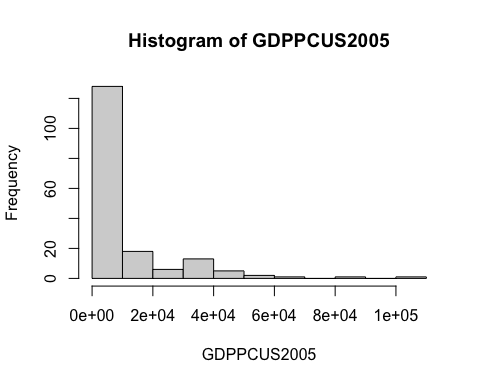
\includegraphics{Assignment1_RMD_files/figure-latex/Question No.6-1.pdf}

\begin{Shaded}
\begin{Highlighting}[]
\FunctionTok{hist}\NormalTok{(}\FunctionTok{log}\NormalTok{(GDPPCUS2005))}
\end{Highlighting}
\end{Shaded}

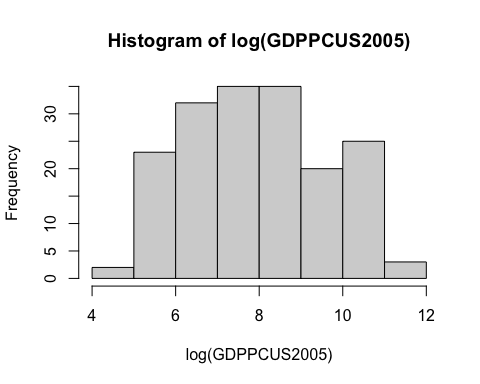
\includegraphics{Assignment1_RMD_files/figure-latex/Question No.6-2.pdf}

\begin{Shaded}
\begin{Highlighting}[]
\FunctionTok{hist}\NormalTok{(HXPC2005)}
\end{Highlighting}
\end{Shaded}

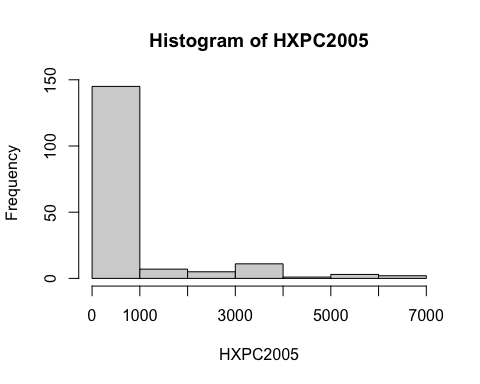
\includegraphics{Assignment1_RMD_files/figure-latex/Question No.6-3.pdf}

\begin{Shaded}
\begin{Highlighting}[]
\FunctionTok{hist}\NormalTok{(}\FunctionTok{log}\NormalTok{(HXPC2005))}
\end{Highlighting}
\end{Shaded}

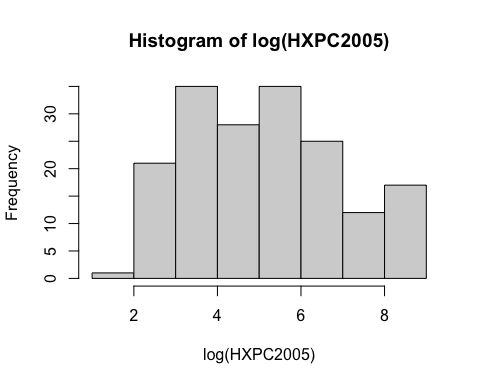
\includegraphics{Assignment1_RMD_files/figure-latex/Question No.6-4.pdf}

\begin{Shaded}
\begin{Highlighting}[]
\FunctionTok{hist}\NormalTok{(LEBF20052)}
\end{Highlighting}
\end{Shaded}

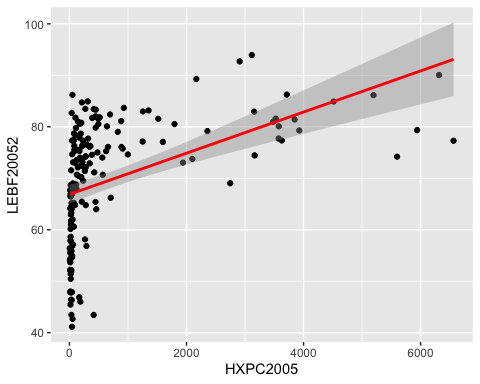
\includegraphics{Assignment1_RMD_files/figure-latex/Question No.6-5.pdf}

\begin{Shaded}
\begin{Highlighting}[]
\FunctionTok{ggplot}\NormalTok{(Dataset1, }\FunctionTok{aes}\NormalTok{(}\AttributeTok{x =}\NormalTok{ HXPC2005, }\AttributeTok{y =}\NormalTok{ LEBF20052)) }\SpecialCharTok{+} 
  \FunctionTok{geom\_point}\NormalTok{() }\SpecialCharTok{+}
  \FunctionTok{stat\_smooth}\NormalTok{(}\AttributeTok{method =} \StringTok{"lm"}\NormalTok{, }\AttributeTok{col =} \StringTok{"red"}\NormalTok{)}
\end{Highlighting}
\end{Shaded}

\begin{verbatim}
## `geom_smooth()` using formula 'y ~ x'
\end{verbatim}

\begin{verbatim}
## Warning: Removed 1 rows containing non-finite values (stat_smooth).
\end{verbatim}

\begin{verbatim}
## Warning: Removed 1 rows containing missing values (geom_point).
\end{verbatim}

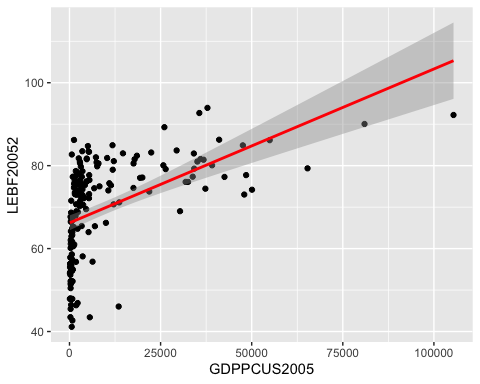
\includegraphics{Assignment1_RMD_files/figure-latex/Question No.6-6.pdf}

\begin{Shaded}
\begin{Highlighting}[]
\FunctionTok{ggplot}\NormalTok{(Dataset1, }\FunctionTok{aes}\NormalTok{(}\AttributeTok{x =}\NormalTok{ GDPPCUS2005, }\AttributeTok{y =}\NormalTok{ LEBF20052)) }\SpecialCharTok{+} 
  \FunctionTok{geom\_point}\NormalTok{() }\SpecialCharTok{+}
  \FunctionTok{stat\_smooth}\NormalTok{(}\AttributeTok{method =} \StringTok{"lm"}\NormalTok{, }\AttributeTok{col =} \StringTok{"red"}\NormalTok{)}
\end{Highlighting}
\end{Shaded}

\begin{verbatim}
## `geom_smooth()` using formula 'y ~ x'
\end{verbatim}

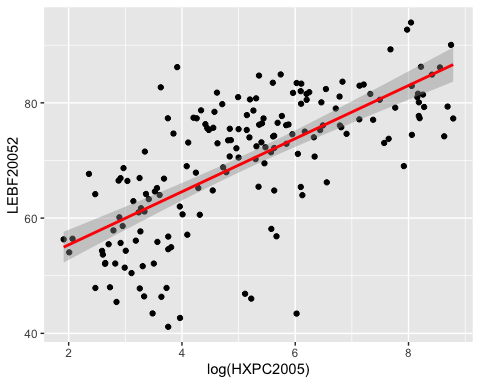
\includegraphics{Assignment1_RMD_files/figure-latex/Question No.6-7.pdf}

\begin{Shaded}
\begin{Highlighting}[]
\FunctionTok{ggplot}\NormalTok{(Dataset1, }\FunctionTok{aes}\NormalTok{(}\AttributeTok{x =} \FunctionTok{log}\NormalTok{(HXPC2005), }\AttributeTok{y =}\NormalTok{ LEBF20052)) }\SpecialCharTok{+} 
  \FunctionTok{geom\_point}\NormalTok{() }\SpecialCharTok{+}
  \FunctionTok{stat\_smooth}\NormalTok{(}\AttributeTok{method =} \StringTok{"lm"}\NormalTok{, }\AttributeTok{col =} \StringTok{"red"}\NormalTok{)}
\end{Highlighting}
\end{Shaded}

\begin{verbatim}
## `geom_smooth()` using formula 'y ~ x'
\end{verbatim}

\begin{verbatim}
## Warning: Removed 1 rows containing non-finite values (stat_smooth).
## Removed 1 rows containing missing values (geom_point).
\end{verbatim}

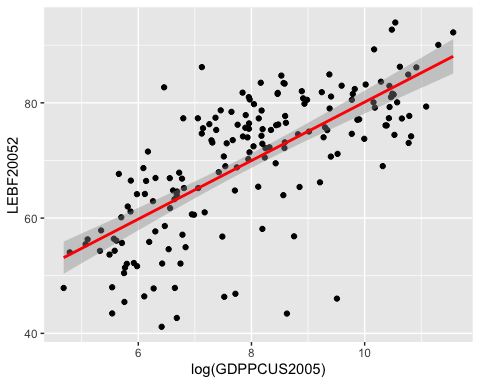
\includegraphics{Assignment1_RMD_files/figure-latex/Question No.6-8.pdf}

\begin{Shaded}
\begin{Highlighting}[]
\FunctionTok{ggplot}\NormalTok{(Dataset1, }\FunctionTok{aes}\NormalTok{(}\AttributeTok{x =} \FunctionTok{log}\NormalTok{(GDPPCUS2005), }\AttributeTok{y =}\NormalTok{ LEBF20052)) }\SpecialCharTok{+} 
  \FunctionTok{geom\_point}\NormalTok{() }\SpecialCharTok{+}
  \FunctionTok{stat\_smooth}\NormalTok{(}\AttributeTok{method =} \StringTok{"lm"}\NormalTok{, }\AttributeTok{col =} \StringTok{"red"}\NormalTok{)}
\end{Highlighting}
\end{Shaded}

\begin{verbatim}
## `geom_smooth()` using formula 'y ~ x'
\end{verbatim}

\includegraphics{Assignment1_RMD_files/figure-latex/Question No.6-9.pdf}
The histograms of GDPPC and HXPC show that their data is rightly skewed
and thus is likely to produce outliers. Additionally, looking at how
well the observations fit around the regression line, we can see that
the plots for both GDDPC and HXPC do not fit the regression line well.
We recommend, doing a log transformation of these two variables because
it will make the big observations in the data smaller and thus closer to
the other variables in the data. This will help reduce the skew and help
the model behave more effectively.The histograms of the log transformed
variables show that when a log transformation is performed the data
approximately fits a normal distribution which is helpful for drawing
statistical inference. The plots for both log(GDDPC) and log(HXPC) also
add support for the use of a log transformation. These plots show that
the regression line fits the data a lot better when these variables are
transformed and thus a non-linear transformation should be used. We
decided to leave LEBF as is because when we look at the histogram for
LEBF the data does not produce an exaggerated skew which is indicative
that the data is okay to work with, without a transformation.

\begin{Shaded}
\begin{Highlighting}[]
\NormalTok{third\_regression }\OtherTok{\textless{}{-}} \FunctionTok{lm}\NormalTok{(LEBF20052}\SpecialCharTok{\textasciitilde{}}\FunctionTok{log}\NormalTok{(HXPC2005)}\SpecialCharTok{+}\FunctionTok{log}\NormalTok{(GDPPCUS2005), Dataset1)}
\NormalTok{Regression\_table3 }\OtherTok{\textless{}{-}} \FunctionTok{msummary}\NormalTok{(}\FunctionTok{list}\NormalTok{(}\StringTok{"non\_log\_reg"} \OtherTok{=}\NormalTok{second\_regression, }
                                   \StringTok{"log\_reg"}\OtherTok{=}\NormalTok{ third\_regression), }
                              \AttributeTok{stars=}\FunctionTok{c}\NormalTok{(}\StringTok{\textquotesingle{}*\textquotesingle{}} \OtherTok{=}\NormalTok{ .}\DecValTok{1}\NormalTok{, }\StringTok{\textquotesingle{}**\textquotesingle{}} \OtherTok{=}\NormalTok{ .}\DecValTok{05}\NormalTok{, }\StringTok{\textquotesingle{}***\textquotesingle{}} \OtherTok{=}\NormalTok{ .}\DecValTok{01}\NormalTok{),}
                              \AttributeTok{fmt =} \StringTok{"\%.4f"}\NormalTok{,  }\AttributeTok{statistic =} \FunctionTok{c}\NormalTok{(}\StringTok{"conf.int"}\NormalTok{,  }\StringTok{"standard error }
\StringTok{                                                           =\{std.error\}"}\NormalTok{, }
                                            \StringTok{"p{-}value = \{p.value\}"}\NormalTok{))}
\NormalTok{Regression\_table3}
\end{Highlighting}
\end{Shaded}

\begin{table}
\centering
\begin{tabular}[t]{lcc}
\toprule
  & non\_log\_reg & log\_reg\\
\midrule
(Intercept) & \num{65.8285}*** & \num{32.4475}***\\
 & {}[\num{63.9781}, \num{67.6788}] & {}[\num{20.8804}, \num{44.0146}]\\
 & standard error 
=\num{0.9374} & standard error 
=\num{5.8599}\\
 & p-value = \num{0.0000} & p-value = \num{0.0000}\\
HXPC2005 & \num{-0.0014} & \\
 & {}[\num{-0.0048}, \num{0.0020}] & \\
 & standard error 
=\num{0.0017} & \\
 & p-value = \num{0.4128} & \\
GDPPCUS2005 & \num{0.0005}*** & \\
 & {}[\num{0.0002}, \num{0.0008}] & \\
 & standard error 
=\num{0.0002} & \\
 & p-value = \num{0.0010} & \\
log(HXPC2005) &  & \num{0.8886}\\
 &  & {}[\num{-2.1532}, \num{3.9305}]\\
 &  & standard error 
=\num{1.5410}\\
 &  & p-value = \num{0.5649}\\
log(GDPPCUS2005) &  & \num{4.1144}**\\
 &  & {}[\num{0.8436}, \num{7.3853}]\\
 &  & standard error 
=\num{1.6570}\\
 &  & p-value = \num{0.0140}\\
\midrule
Num.Obs. & \num{174} & \num{174}\\
R2 & \num{0.252} & \num{0.493}\\
R2 Adj. & \num{0.243} & \num{0.487}\\
AIC & \num{1309.1} & \num{1241.5}\\
BIC & \num{1321.8} & \num{1254.1}\\
Log.Lik. & \num{-650.574} & \num{-616.726}\\
F & \num{28.813} & \num{83.179}\\
RMSE & \num{10.18} & \num{8.38}\\
\bottomrule
\multicolumn{3}{l}{\rule{0pt}{1em}* p $<$ 0.1, ** p $<$ 0.05, *** p $<$ 0.01}\\
\end{tabular}
\end{table}

Applying a non-linear transformation is necessary in order to reduce the
extreme effects of outliers on our regression outputs. Log transforming
the predictor variables in the regression model is one way in which we
can achieve this. It makes sense to log transform the independent
variables in the model by applying a natural log, as we can directly
compare the regression output to those in (5) as the output stays in the
same units. We are also able to apply the natural log as we do not have
any zero-valued data.

By log transforming both HXPC and GDPPC we are provided with new
regression coefficients. The regression coefficient of log(HXPC2005) is
now 0.8886 which is substantially different than the non-log'd
coefficient -0.0014. The new regression coefficient indicates that for
every 10\% increase in HXPC (when GDPPC is held constant), the LEBF will
increase by 0.089. Intuitively, life expectancy should increase as there
is more health expenditure within a country so these new results make
more sense which speaks to the value of transforming the HXPC variable.
The results however remain statistically insignificant. The regression
coefficient for log(GDPPCUS2005) also changed to 4.114 which is an
increase from the non-log'd coefficient of 0.0005. Both coefficients
were deemed as statistically significant. The new regression coefficient
indicates that for every 10\% increase in GDP (when HXPC is held
constant) there is a 0.4114 unit (year) increase in life expectancy at
birth for females. We can also see that the R\^{}2 value has increased
from 0.252 to 0.493 which indicates that the new regression line fits
better to the data.

\begin{center}\rule{0.5\linewidth}{0.5pt}\end{center}

Question 7 - How might these results differ by geography? Create a
variable that assigns each observation to a geographic region (e.g.,
continent) and report a regression that builds on (6) by including the
appropriate dummy variables. Interpret your results.

\begin{Shaded}
\begin{Highlighting}[]
\NormalTok{Dataset1}\SpecialCharTok{$}\NormalTok{continent }\OtherTok{\textless{}{-}} \FunctionTok{countrycode}\NormalTok{(}\AttributeTok{sourcevar =}\NormalTok{ Dataset1[,}\StringTok{"Country"}\NormalTok{],}
                                      \AttributeTok{origin =} \StringTok{"country.name"}\NormalTok{,}
                                   \AttributeTok{destination =} \StringTok{"continent"}\NormalTok{)}

\FunctionTok{view}\NormalTok{(Dataset1)}
\FunctionTok{unique}\NormalTok{(Dataset1[}\FunctionTok{c}\NormalTok{(}\StringTok{"continent"}\NormalTok{)])}
\end{Highlighting}
\end{Shaded}

\begin{verbatim}
##   continent
## 1      Asia
## 2    Europe
## 3    Africa
## 5  Americas
## 7   Oceania
\end{verbatim}

\begin{Shaded}
\begin{Highlighting}[]
\CommentTok{\#the country code package grouped North and South America into the Americas}

\NormalTok{Dataset1 }\OtherTok{\textless{}{-}} \FunctionTok{dummy\_cols}\NormalTok{(Dataset1, }\AttributeTok{select\_columns =} \StringTok{"continent"}\NormalTok{) }\CommentTok{\#used fast dummies to make dummy variables}

\NormalTok{continet\_regression }\OtherTok{\textless{}{-}} \FunctionTok{lm}\NormalTok{(LEBF20052}\SpecialCharTok{\textasciitilde{}}\FunctionTok{log}\NormalTok{(HXPC2005)}\SpecialCharTok{+}\FunctionTok{log}\NormalTok{(GDPPCUS2005) }\SpecialCharTok{+}\NormalTok{ continent\_Africa }\SpecialCharTok{+}
\NormalTok{                            continent\_Americas }\SpecialCharTok{+}\NormalTok{ continent\_Asia }\SpecialCharTok{+}\NormalTok{ continent\_Europe}
                          \SpecialCharTok{+}\NormalTok{ continent\_Oceania, Dataset1)}
\CommentTok{\#all dummy variables are in the regression {-} to let R decide which one to drop (R decided to drop Oceania) to avoid the dummy variable trap}

\NormalTok{Regression\_table4 }\OtherTok{\textless{}{-}} \FunctionTok{msummary}\NormalTok{(}\FunctionTok{list}\NormalTok{(}\StringTok{"continent\_reg"}\OtherTok{=}\NormalTok{continet\_regression),}
                              \AttributeTok{stars=}\FunctionTok{c}\NormalTok{(}\StringTok{\textquotesingle{}*\textquotesingle{}} \OtherTok{=}\NormalTok{ .}\DecValTok{1}\NormalTok{, }\StringTok{\textquotesingle{}**\textquotesingle{}} \OtherTok{=}\NormalTok{ .}\DecValTok{05}\NormalTok{, }\StringTok{\textquotesingle{}***\textquotesingle{}} \OtherTok{=}\NormalTok{ .}\DecValTok{01}\NormalTok{),}
                               \AttributeTok{fmt =} \DecValTok{5}\NormalTok{,  }\AttributeTok{statistic =} \FunctionTok{c}\NormalTok{(}\StringTok{"conf.int"}\NormalTok{,  }\StringTok{"standard error = \{std.error\}"}\NormalTok{, }
                                            \StringTok{"p{-}value = \{p.value\}"}\NormalTok{))}
\NormalTok{Regression\_table4}
\end{Highlighting}
\end{Shaded}

\begin{table}
\centering
\begin{tabular}[t]{lc}
\toprule
  & continent\_reg\\
\midrule
(Intercept) & \num{45.17849}***\\
 & {}[\num{33.76678}, \num{56.59020}]\\
 & standard error = \num{5.78021}\\
 & p-value = \num{0.00000}\\
log(HXPC2005) & \num{0.08624}\\
 & {}[\num{-2.77520}, \num{2.94768}]\\
 & standard error = \num{1.44937}\\
 & p-value = \num{0.95262}\\
log(GDPPCUS2005) & \num{3.31976}**\\
 & {}[\num{0.39577}, \num{6.24374}]\\
 & standard error = \num{1.48104}\\
 & p-value = \num{0.02631}\\
continent\_Africa & \num{-10.33203}***\\
 & {}[\num{-15.62039}, \num{-5.04366}]\\
 & standard error = \num{2.67864}\\
 & p-value = \num{0.00016}\\
continent\_Americas & \num{1.83521}\\
 & {}[\num{-3.58536}, \num{7.25578}]\\
 & standard error = \num{2.74561}\\
 & p-value = \num{0.50479}\\
continent\_Asia & \num{1.24018}\\
 & {}[\num{-3.98199}, \num{6.46235}]\\
 & standard error = \num{2.64511}\\
 & p-value = \num{0.63978}\\
continent\_Europe & \num{0.69582}\\
 & {}[\num{-4.80230}, \num{6.19393}]\\
 & standard error = \num{2.78488}\\
 & p-value = \num{0.80301}\\
\midrule
Num.Obs. & \num{174}\\
R2 & \num{0.641}\\
R2 Adj. & \num{0.628}\\
AIC & \num{1189.6}\\
BIC & \num{1214.9}\\
Log.Lik. & \num{-586.794}\\
RMSE & \num{7.05}\\
\bottomrule
\multicolumn{2}{l}{\rule{0pt}{1em}* p $<$ 0.1, ** p $<$ 0.05, *** p $<$ 0.01}\\
\end{tabular}
\end{table}

When including variables that assign each observation to a geographic
region (and holding them constant), the relationship between HXPC and
LEBF (when GDPPC is held constant) shows a 10\% increase in HXPC is
associated with a 0.0086 increase in LEBF, but this remains not
statistically significant. The relationship between GDPPC and LEBF (when
HXPC is held constant) sees a 10\% increase in GDDPC significantly
associated with a 0.33 increase in LEBF which is a slight decrease from
the output reported in (6) where a 10\% increase in GDDPC was
significantly associated with a 0.4114 increase in LEBF. The results of
our model also demonstrate that when continent dummy variables are
included, the OLS line experiences intercept shifts that are contingent
on what continent is being examined. The association between the
continent of Africa and LEBF (when controlling for HXPC, GDDPC, and
other continents) is statistically significant and has a negative
intercept shift (vs.~Oceania). Conversely, the other continents have
positive intercept shifts with LEBF (vs.~Oceania) although their
regression coefficients are not statistically significant. The R\^{}2
for the model of 0.641 shows good model fit and indicates that the
variables in the model are able to adequately account for the variation
in LEBF.

\begin{center}\rule{0.5\linewidth}{0.5pt}\end{center}

Question 8 - Finally, include an interaction term between HXPC and the
indicator for African countries. What are you measuring with this
interaction, and why might it be meaningful? Interpret the results of
this coefficient.

\begin{Shaded}
\begin{Highlighting}[]
\NormalTok{interaction\_regression }\OtherTok{\textless{}{-}} \FunctionTok{lm}\NormalTok{(LEBF20052}\SpecialCharTok{\textasciitilde{}}\FunctionTok{log}\NormalTok{(HXPC2005) }
                          \SpecialCharTok{+}\FunctionTok{log}\NormalTok{(GDPPCUS2005) }
                          \SpecialCharTok{+}\NormalTok{ continent\_Africa }
                          \SpecialCharTok{+}\NormalTok{ continent\_Americas }
                          \SpecialCharTok{+}\NormalTok{ continent\_Asia }
                          \SpecialCharTok{+}\NormalTok{ continent\_Europe}
                          \SpecialCharTok{+}\NormalTok{ continent\_Oceania }
                          \SpecialCharTok{+} \FunctionTok{log}\NormalTok{(HXPC2005)}\SpecialCharTok{:}\NormalTok{continent\_Africa, Dataset1)}

\NormalTok{Regression\_table5 }\OtherTok{\textless{}{-}} \FunctionTok{msummary}\NormalTok{(}\FunctionTok{list}\NormalTok{(}\StringTok{"interaction\_reg"}\OtherTok{=}\NormalTok{interaction\_regression),}
                              \AttributeTok{stars=}\FunctionTok{c}\NormalTok{(}\StringTok{\textquotesingle{}*\textquotesingle{}} \OtherTok{=}\NormalTok{ .}\DecValTok{1}\NormalTok{, }\StringTok{\textquotesingle{}**\textquotesingle{}} \OtherTok{=}\NormalTok{ .}\DecValTok{05}\NormalTok{, }\StringTok{\textquotesingle{}***\textquotesingle{}} \OtherTok{=}\NormalTok{ .}\DecValTok{01}\NormalTok{),}
                              \AttributeTok{fmt =} \DecValTok{5}\NormalTok{,  }\AttributeTok{statistic =} \FunctionTok{c}\NormalTok{(}\StringTok{"conf.int"}\NormalTok{,  }
                                                      \StringTok{"standard error = \{std.error\}"}\NormalTok{, }
                                            \StringTok{"p{-}value = \{p.value\}"}\NormalTok{))}


\NormalTok{Regression\_table5}
\end{Highlighting}
\end{Shaded}

\begin{table}
\centering
\begin{tabular}[t]{lc}
\toprule
  & interaction\_reg\\
\midrule
(Intercept) & \num{45.73991}***\\
 & {}[\num{33.76584}, \num{57.71398}]\\
 & standard error = \num{6.06479}\\
 & p-value = \num{0.00000}\\
log(HXPC2005) & \num{0.06629}\\
 & {}[\num{-2.80577}, \num{2.93834}]\\
 & standard error = \num{1.45468}\\
 & p-value = \num{0.96371}\\
log(GDPPCUS2005) & \num{3.26349}**\\
 & {}[\num{0.31024}, \num{6.21674}]\\
 & standard error = \num{1.49580}\\
 & p-value = \num{0.03053}\\
continent\_Africa & \num{-11.62631}**\\
 & {}[\num{-21.33206}, \num{-1.92056}]\\
 & standard error = \num{4.91590}\\
 & p-value = \num{0.01918}\\
continent\_Americas & \num{1.85270}\\
 & {}[\num{-3.58390}, \num{7.28930}]\\
 & standard error = \num{2.75361}\\
 & p-value = \num{0.50199}\\
continent\_Asia & \num{1.21749}\\
 & {}[\num{-4.02099}, \num{6.45598}]\\
 & standard error = \num{2.65326}\\
 & p-value = \num{0.64693}\\
continent\_Europe & \num{0.80760}\\
 & {}[\num{-4.75017}, \num{6.36536}]\\
 & standard error = \num{2.81498}\\
 & p-value = \num{0.77455}\\
log(HXPC2005) × continent\_Africa & \num{0.31885}\\
 & {}[\num{-1.68374}, \num{2.32144}]\\
 & standard error = \num{1.01430}\\
 & p-value = \num{0.75365}\\
\midrule
Num.Obs. & \num{174}\\
R2 & \num{0.641}\\
R2 Adj. & \num{0.626}\\
AIC & \num{1191.5}\\
BIC & \num{1219.9}\\
Log.Lik. & \num{-586.742}\\
RMSE & \num{7.05}\\
\bottomrule
\multicolumn{2}{l}{\rule{0pt}{1em}* p $<$ 0.1, ** p $<$ 0.05, *** p $<$ 0.01}\\
\end{tabular}
\end{table}

With this interaction term we are measuring the effect of HXPC specific
to African countries. It might be meaningful to include this interaction
term as it would allow us to determine how much stronger the effect of
HXPC on LEBF is when the continent is Africa. When we look at the
interaction between HXPC and the continent of Africa we see that the
regression coefficient is 0.32, which indicates that for Africa, a 10\%
increase in health expenditure leads to an additional 0.032 life years
on top of the general effect of health expenditure which would be 0.0066
life years for ever 10\% increase in health expenditure (regression
coefficient of HXPC is 0.06629). It is the combination of these two
values that lets us identify that the effect of a 10\% increase in
health expenditure in Africa increases LEBF by 0.0385 units (years). It
must be noted that these regression coefficients were not statistically
significant.

\begin{center}\rule{0.5\linewidth}{0.5pt}\end{center}

Question 9 - Why is establishing the causal relationship between GDDPC,
HXPC, and LEBF difficult in a simple regression such as this? If
possible, provide one key figure that highlights an identification
problem in this scenario. (Note that there are multiple possible answers
for this problem; the goal is to think critically about the causal
identification.)

\begin{Shaded}
\begin{Highlighting}[]
\NormalTok{q}\FloatTok{.9}\NormalTok{\_regression}\FloatTok{.1} \OtherTok{\textless{}{-}} \FunctionTok{lm}\NormalTok{(LEBF20052}\SpecialCharTok{\textasciitilde{}}\FunctionTok{log}\NormalTok{(GDPPCUS2005), Dataset1)}
\NormalTok{q}\FloatTok{.9}\NormalTok{\_regression}\FloatTok{.2} \OtherTok{\textless{}{-}} \FunctionTok{lm}\NormalTok{(LEBF20052}\SpecialCharTok{\textasciitilde{}}\FunctionTok{log}\NormalTok{(HXPC2005), Dataset1)}

\NormalTok{q}\FloatTok{.9}\NormalTok{\_table }\OtherTok{\textless{}{-}} \FunctionTok{msummary}\NormalTok{(}\FunctionTok{list}\NormalTok{(}\StringTok{"LEBF\_log(GDP)"}\OtherTok{=}\NormalTok{q}\FloatTok{.9}\NormalTok{\_regression}\FloatTok{.1}\NormalTok{, }\StringTok{"LEBF\_log(HXPC)"}\OtherTok{=}\NormalTok{q}\FloatTok{.9}\NormalTok{\_regression}\FloatTok{.2}\NormalTok{,}
                           \StringTok{"LEBF\_log(GDP)+log(HXPC)"}\OtherTok{=}\NormalTok{ third\_regression), }\AttributeTok{fmt =} \StringTok{"\%.4f"}\NormalTok{,}
                      \AttributeTok{stars=}\FunctionTok{c}\NormalTok{(}\StringTok{\textquotesingle{}*\textquotesingle{}} \OtherTok{=}\NormalTok{ .}\DecValTok{1}\NormalTok{, }\StringTok{\textquotesingle{}**\textquotesingle{}} \OtherTok{=}\NormalTok{ .}\DecValTok{05}\NormalTok{, }\StringTok{\textquotesingle{}***\textquotesingle{}} \OtherTok{=}\NormalTok{ .}\DecValTok{01}\NormalTok{),  }
                      \AttributeTok{statistic =} \FunctionTok{c}\NormalTok{(}\StringTok{"conf.int"}\NormalTok{, }\StringTok{"standard error = \{std.error\}"}\NormalTok{, }
                                            \StringTok{"p{-}value = \{p.value\}"}\NormalTok{))  }

\NormalTok{q}\FloatTok{.9}\NormalTok{\_table}
\end{Highlighting}
\end{Shaded}

\begin{table}
\centering
\begin{tabular}[t]{lccc}
\toprule
  & LEBF\_log(GDP) & LEBF\_log(HXPC) & LEBF\_log(GDP)+log(HXPC)\\
\midrule
(Intercept) & \num{29.3770}*** & \num{46.1508}*** & \num{32.4475}***\\
 & {}[\num{23.1953}, \num{35.5588}] & {}[\num{42.2044}, \num{50.0973}] & {}[\num{20.8804}, \num{44.0146}]\\
 & standard error = \num{3.1320} & standard error = \num{1.9994} & standard error = \num{5.8599}\\
 & p-value = \num{0.0000} & p-value = \num{0.0000} & p-value = \num{0.0000}\\
log(GDPPCUS2005) & \num{5.0751}*** &  & \num{4.1144}**\\
 & {}[\num{4.3162}, \num{5.8339}] &  & {}[\num{0.8436}, \num{7.3853}]\\
 & standard error = \num{0.3845} &  & standard error = \num{1.6570}\\
 & p-value = \num{0.0000} &  & p-value = \num{0.0140}\\
log(HXPC2005) &  & \num{4.6067}*** & \num{0.8886}\\
 &  & {}[\num{3.8776}, \num{5.3358}] & {}[\num{-2.1532}, \num{3.9305}]\\
 &  & standard error = \num{0.3694} & standard error = \num{1.5410}\\
 &  & p-value = \num{0.0000} & p-value = \num{0.5649}\\
\midrule
Num.Obs. & \num{175} & \num{174} & \num{174}\\
R2 & \num{0.502} & \num{0.475} & \num{0.493}\\
R2 Adj. & \num{0.499} & \num{0.472} & \num{0.487}\\
AIC & \num{1246.1} & \num{1245.6} & \num{1241.5}\\
BIC & \num{1255.6} & \num{1255.1} & \num{1254.1}\\
Log.Lik. & \num{-620.066} & \num{-619.807} & \num{-616.726}\\
F & \num{174.249} & \num{155.523} & \num{83.179}\\
RMSE & \num{8.37} & \num{8.53} & \num{8.38}\\
\bottomrule
\multicolumn{4}{l}{\rule{0pt}{1em}* p $<$ 0.1, ** p $<$ 0.05, *** p $<$ 0.01}\\
\end{tabular}
\end{table}

Establishing the causal relationship between GDDPC, HXPC, and LEBF in a
simple regression such as this is difficult as there are many sources of
variation that can complicate the causal pathway between these three
variables (as shown in the DAG in Question 1). This relationship is
further complicated when the relationship between continents (countries)
are taken into consideration, as from our DAG they drive much of the
variation seen within GDPPC and subsequently HXPC.From our DAG we can
see a substantial number of different sources of variation coming from
GDPPC (which ultimately includes HXPC). Both GDPPC and HXPC account for
a substantial amount of variation in LEBF (when we examine R\^{}2 in the
regressions for both explanatory variables on LEBF), but using theory
(seen through our DAG) we can realize that there are other contributors
within the data generating process that are not captured through this
relationship. Additionally, when constructing a bivariate model, we can
see that the R\^{}2 is still lower than the univariate model examining
LEBF and GDPPC, indicating that the inclusion of HXPC does not help in
identifying what is associated with variation in LEBF. Moreover in this
bivariate model, when controlling for GDPPC, HXPC decreases
substantially from the univariate (LEBF\textasciitilde HXPC) model and
becomes statistically insignificant. This indicates that HXPC likely has
a much smaller role to play in the relationship between HXPC, GDPPC, and
LEBF when GDPPC is taken into consideration. From this, we can
appreciate that the DAG can help us to form testable assumptions and the
models can help us to check those assumptions (to a point), but
ultimately unless we are certain that we have accounted for all the
variation in our outcome (through the DAG we construct), we cannot
establish a causal relationship between HXPC, GDPPC, and LEBF.

\begin{center}\rule{0.5\linewidth}{0.5pt}\end{center}

Question 10 - What do your results from (9) and intuition suggest about
the standard errors in your specification? Either justify the use of
homoscedastic standard errors or implement a full specification with
another, more robust method (e.g., heteroskedasticity-robust or
clustered SEs). How does this change the results?

\begin{Shaded}
\begin{Highlighting}[]
\CommentTok{\#plot the residuals vs fitted values}
\FunctionTok{par}\NormalTok{(}\AttributeTok{mfrow =} \FunctionTok{c}\NormalTok{(}\DecValTok{2}\NormalTok{, }\DecValTok{2}\NormalTok{))}
\FunctionTok{plot}\NormalTok{(interaction\_regression)}
\end{Highlighting}
\end{Shaded}

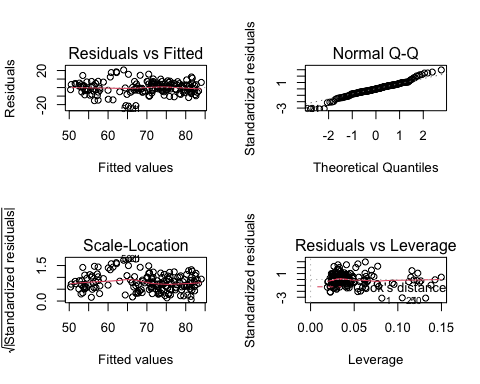
\includegraphics{Assignment1_RMD_files/figure-latex/Question No.10-1.pdf}

\begin{Shaded}
\begin{Highlighting}[]
\CommentTok{\#plot shows heteroskedasticity may exist}

\CommentTok{\#Breusch{-}Pagan test for heteroskedasticity }

\NormalTok{lmtest}\SpecialCharTok{::}\FunctionTok{bptest}\NormalTok{(interaction\_regression)}
\end{Highlighting}
\end{Shaded}

\begin{verbatim}
## 
##  studentized Breusch-Pagan test
## 
## data:  interaction_regression
## BP = 49.788, df = 7, p-value = 1.59e-08
\end{verbatim}

\begin{Shaded}
\begin{Highlighting}[]
\CommentTok{\#the bptest is showing that the we can reject the null that the residuals are distributed with equal variance (homoscedasticty) as there is a high test statistic (BP = 49.79) and a p value \textless{} 0.05, therefore we can reject the null that the residuals are homoscedastic}


\CommentTok{\#specification using both robust corrections for standard errors and autocorrelation}
\NormalTok{se\_corrections}\OtherTok{\textless{}{-}} \FunctionTok{msummary}\NormalTok{(}\FunctionTok{list}\NormalTok{(}\StringTok{"homoscedastic"} \OtherTok{=}\NormalTok{ interaction\_regression,}
                               \StringTok{"robust\_se"} \OtherTok{=}\NormalTok{interaction\_regression),}
          \AttributeTok{stars=}\FunctionTok{c}\NormalTok{(}\StringTok{\textquotesingle{}*\textquotesingle{}} \OtherTok{=}\NormalTok{ .}\DecValTok{1}\NormalTok{, }\StringTok{\textquotesingle{}**\textquotesingle{}} \OtherTok{=}\NormalTok{ .}\DecValTok{05}\NormalTok{, }\StringTok{\textquotesingle{}***\textquotesingle{}} \OtherTok{=}\NormalTok{ .}\DecValTok{01}\NormalTok{), }
          \AttributeTok{vcov =}\FunctionTok{c}\NormalTok{(}\StringTok{"classical"}\NormalTok{,}\StringTok{"robust"}\NormalTok{),}
          \AttributeTok{fmt =} \StringTok{"\%.2f"}\NormalTok{, }\AttributeTok{statistic =} \FunctionTok{c}\NormalTok{(}\StringTok{"conf.int"}\NormalTok{, }\StringTok{"standard error = \{std.error\}"}\NormalTok{, }
                                            \StringTok{"p{-}value = \{p.value\}"}\NormalTok{))}

\NormalTok{se\_corrections}
\end{Highlighting}
\end{Shaded}

\begin{table}
\centering
\begin{tabular}[t]{lcc}
\toprule
  & homoscedastic & robust\_se\\
\midrule
(Intercept) & \num{45.74}*** & \num{45.74}***\\
 & {}[\num{33.77}, \num{57.71}] & {}[\num{29.23}, \num{62.25}]\\
 & standard error = \num{6.06} & standard error = \num{8.36}\\
 & p-value = \num{0.00} & p-value = \num{0.00}\\
log(HXPC2005) & \num{0.07} & \num{0.07}\\
 & {}[\num{-2.81}, \num{2.94}] & {}[\num{-4.01}, \num{4.14}]\\
 & standard error = \num{1.45} & standard error = \num{2.06}\\
 & p-value = \num{0.96} & p-value = \num{0.97}\\
log(GDPPCUS2005) & \num{3.26}** & \num{3.26}\\
 & {}[\num{0.31}, \num{6.22}] & {}[\num{-1.23}, \num{7.76}]\\
 & standard error = \num{1.50} & standard error = \num{2.28}\\
 & p-value = \num{0.03} & p-value = \num{0.15}\\
continent\_Africa & \num{-11.63}** & \num{-11.63}**\\
 & {}[\num{-21.33}, \num{-1.92}] & {}[\num{-22.58}, \num{-0.67}]\\
 & standard error = \num{4.92} & standard error = \num{5.55}\\
 & p-value = \num{0.02} & p-value = \num{0.04}\\
continent\_Americas & \num{1.85} & \num{1.85}\\
 & {}[\num{-3.58}, \num{7.29}] & {}[\num{-2.01}, \num{5.72}]\\
 & standard error = \num{2.75} & standard error = \num{1.96}\\
 & p-value = \num{0.50} & p-value = \num{0.35}\\
continent\_Asia & \num{1.22} & \num{1.22}\\
 & {}[\num{-4.02}, \num{6.46}] & {}[\num{-2.79}, \num{5.23}]\\
 & standard error = \num{2.65} & standard error = \num{2.03}\\
 & p-value = \num{0.65} & p-value = \num{0.55}\\
continent\_Europe & \num{0.81} & \num{0.81}\\
 & {}[\num{-4.75}, \num{6.37}] & {}[\num{-3.19}, \num{4.81}]\\
 & standard error = \num{2.81} & standard error = \num{2.02}\\
 & p-value = \num{0.77} & p-value = \num{0.69}\\
log(HXPC2005) × continent\_Africa & \num{0.32} & \num{0.32}\\
 & {}[\num{-1.68}, \num{2.32}] & {}[\num{-2.75}, \num{3.39}]\\
 & standard error = \num{1.01} & standard error = \num{1.56}\\
 & p-value = \num{0.75} & p-value = \num{0.84}\\
\midrule
Num.Obs. & \num{174} & \num{174}\\
R2 & \num{0.641} & \num{0.641}\\
R2 Adj. & \num{0.626} & \num{0.626}\\
AIC & \num{1191.5} & \num{1191.5}\\
BIC & \num{1219.9} & \num{1219.9}\\
Log.Lik. & \num{-586.742} & \num{-586.742}\\
RMSE & \num{7.05} & \num{7.05}\\
Std.Errors & Classical & Robust\\
\bottomrule
\multicolumn{3}{l}{\rule{0pt}{1em}* p $<$ 0.1, ** p $<$ 0.05, *** p $<$ 0.01}\\
\end{tabular}
\end{table}

The results from question 9, and our intuition suggest that the standard
errors in our specification are not homoscedastic. To check if it is
accurate to use homoscedastic errors, a plot was created to look at the
residual vs fitted values of our model that includes continents. We
include continents to represent our theoretical assumptions outlined in
our DAG, indicating that the variation of GDPPC and HXPC begins from
country (continental) variation. In this residual plot, we can see that
the data is not randomly spread around the 0 line and thus indicative
that the use of homoscedastic standard errors may not be best practice.
To confirm what we saw in the residual vs fitted plot, we conducted a
Breusch-Pagan test to test for heteroskedasticity in our model. The
results of our Breusch-Pagan test displayed a high test statistic and a
p value \textless{} 0.05. Therefore, we reject the null hypothesis and
can confirm that this regression model violates the homoscedasticity
assumption. As a result of this plot and the Breusch-Pagan test, we
implemented a correction for heteroskedasticity within our model. We did
not implement a correction for autocorrelation as our data was not
collected over multiple time periods so it would not make sense for
autocorrelation to have an impact. When we used the
heteroskedasticity-robust method for our standard errors we observed
that the standard errors for log(HXPC) and log(GDPPC) increased from
1.45 and 1.50 to 2.06 and 2.28 respectively. The standard errors
increasing indicates that our standard errors are becoming more accurate
in describing the data. We can also see that within our data that the
regression coefficient for log(GDPPC) is no longer significant after
this method is employed. This result is expected because the larger
standard error, 2.78, observed leads to a test statistic that is
smaller. Smaller test statistics are associated with larger p-values
thus the loss of significance of the regression coefficient for
log(GDDPC) as a result of the heteroskedasticity-robust method employed
makes sense. \#i didnt talk about the other standard errors for the
continents - idk if i should but get some funky things that idk how to
explain like standard errors going down not up haha

\begin{center}\rule{0.5\linewidth}{0.5pt}\end{center}

\end{document}
